
\begin{figure}[H]
	\centering			
	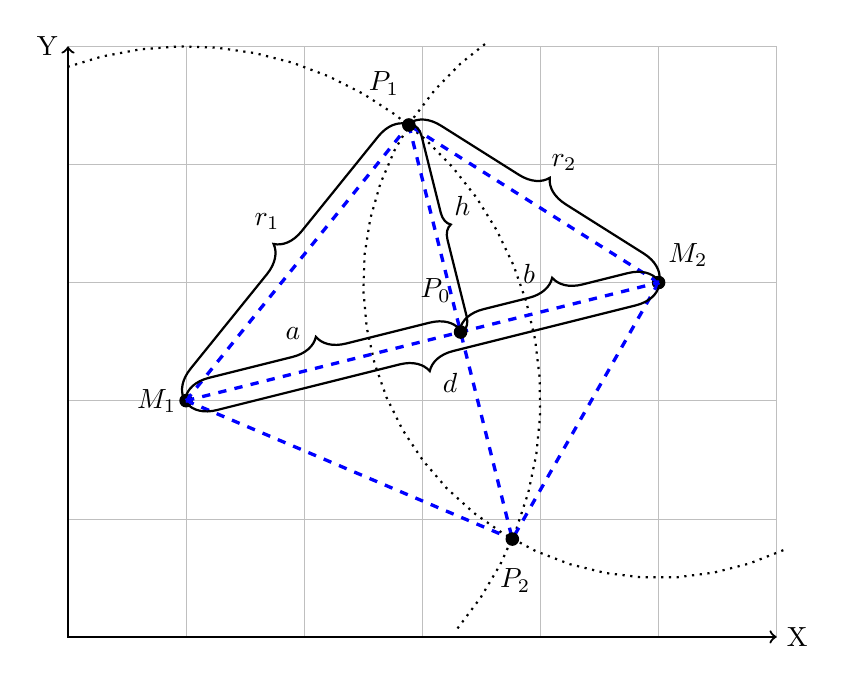
\begin{tikzpicture}[scale=1.5, domain=0:4]
		% grid
      	\draw[very thin,color=lightgray] (0,0) grid (6,5);
      	\draw [<->,thick] (0,5) node (yaxis) [left] {Y} |- (6,0) node (xaxis) [right] {X};

		% Definitions
    	\pgfmathsetlengthmacro{\ra}{3cm}
    	\pgfmathsetlengthmacro{\xa}{1cm}
    	\pgfmathsetlengthmacro{\ya}{2cm}
    
    	\pgfmathsetlengthmacro{\rb}{2.5cm}
    	\pgfmathsetlengthmacro{\xb}{5cm}
    	\pgfmathsetlengthmacro{\yb}{3cm}
	
		% The middlepoints
  		\coordinate (CA) at (\xa,\ya);
  		\coordinate (CB) at (\xb,\yb);
  
  		% The point
  		\draw[fill,color=black] (CA) circle (1.5pt) node[left, color=black] {$M_1$};
  		\draw[fill,color=black] (CB) circle (1.5pt) node[right, yshift=10pt, color=black] {$M_2$};
  
  		% The circle
  		%\draw[dashed,color=black] (CA) circle (\ra);
		%\draw[dashed,color=black] (CB) circle (\rb);
  
		\draw [dotted,thick,domain=-40:110] plot ({1+3*cos(\x)}, {2+3*sin(\x)});
		\draw [dotted,thick,domain=295:125] plot ({5+2.5*cos(\x)}, {3+2.5*sin(\x)});
	
		\coordinate (PA) at (2.885365678957660, 4.333537284169362);
    	\coordinate (PB) at (3.761693144571752, 0.828227421712991);
		\coordinate (PO) at (3.323529411764706, 2.580882352941176);
		
		\draw[very thick,color=blue,dashed] (CA) -- (CB);
      	\draw[very thick,color=blue,dashed] (PA) -- (PB);
      	\draw[very thick,color=blue,dashed] (CA) -- (PA);
      	\draw[very thick,color=blue,dashed] (CA) -- (PB);
      	\draw[very thick,color=blue,dashed] (CB) -- (PA);
      	\draw[very thick,color=blue,dashed] (CB) -- (PB);
      
      	\draw[thick,decorate,decoration={brace,amplitude=5pt,mirror,raise=1pt}] (PO) -- (PA) node[midway,xshift=10pt,yshift=8pt] {$h$};
	
\draw[thick,decorate,decoration={brace,amplitude=10pt,mirror,raise=1pt}] (CA) -- (CB) node[midway,xshift=10pt,yshift=-15pt] {$d$};
      \draw[thick,decorate,decoration={brace,amplitude=10pt,raise=1pt}] (CA) -- (PO) node[midway,xshift=-11pt,yshift=12pt] {$a$};
      \draw[thick,decorate,decoration={brace,amplitude=10pt,raise=1pt}] (PO) -- (CB) node[midway,xshift=-11pt,yshift=12pt] {$b$};	
      
      \draw[thick,decorate,decoration={brace,amplitude=10pt,raise=1pt}] (CA) -- (PA) node[midway,xshift=-11pt,yshift=15pt] {$r_1$};	
      \draw[thick,decorate,decoration={brace,amplitude=10pt,raise=1pt}] (PA) -- (CB) node[midway,xshift=+11pt,yshift=15pt] {$r_2$};	
      
      \draw[fill,color=black] (PA) circle (1.5pt) node[left, yshift=15pt, color=black] {$P_1$};
      \draw[fill,color=black] (PB) circle (1.5pt) node[left, xshift=10pt, yshift=-15pt, color=black] {$P_2$};	
      \draw[fill,color=black] (PO) circle (1.5pt) node[left, yshift=15pt, color=black] {$P_0$};
	
	\end{tikzpicture}
	\caption{Snijpunten van twee cirkels}
  	\label{fig:snijpunten}
\end{figure}
